\documentclass[conference]{IEEEtran}
\IEEEoverridecommandlockouts
% The preceding line is only needed to identify funding in the first footnote. If that is unneeded, please comment it out.
\usepackage{cite}
\usepackage{amsmath,amssymb,amsfonts}
\usepackage{algorithmic}
\usepackage{graphicx}
\usepackage[colorlinks=true, allcolors=blue]{hyperref}
\usepackage{url}
\usepackage{textcomp}
\usepackage{minted}
\usepackage{booktabs}
\usepackage{xcolor}
\usepackage{adjustbox}
\newminted{python}{
    linenos,
    autogobble,
    breaklines,
    fontsize=\scriptsize,
    frame=lines,
    framesep=2mm,
    bgcolor=black!5,
    rulecolor=\color{gray},
    framesep=3mm,
    baselinestretch=1.2,
    tabsize=4,
}
\usepackage[font=small,skip=1pt]{caption}
\captionsetup{skip=-1pt}
\usepackage{subcaption}
\captionsetup[subfigure]{aboveskip=-3pt}
\def\BibTeX{{\rm B\kern-.05em{\sc i\kern-.025em b}\kern-.08em
    T\kern-.1667em\lower.7ex\hbox{E}\kern-.125emX}}
\begin{document}

\title{Predicting 5G Network Slice Types Based on User Requirements and Charactersitics}

\author{\IEEEauthorblockN{Sina Ebrahimi}
\IEEEauthorblockA{\textit{Centre for Future Transport and Cities} \\
\textit{Coventry University}\\
Coventry, UK \\
ebrahimis@coventry.ac.uk}
}

\maketitle

\begin{abstract}
This paper examines a prediction problem that aims to accurately classify the Network Slice (NS) type of mobile end-users based on specific requirements (e.g., packet loss rate and packet delay) and characteristics (such as belonging to a service category). The issue at hand pertains to a forecasting problem with three distinct classes. Another resource allocation scheme in a wireless network, such as 5G, can utilize this prediction model to serve end-users. Initially, we conducted an analysis of the dataset. Subsequently, we employ various classification techniques, namely Decision Tree (DT), Random Forest (RF), K-Nearest Neighbors (KNN), Logistic Regression (LR), and Support Vector Machine (SVM), in order to determine the most suitable method for this particular problem. Upon evaluating the classifiers, it becomes evident that DT, RF, and KNN exhibit a distinct advantage over LR and SVM. The DT model surpasses the RF and KNN models by approximately 1\% and 2\% in all metrics, such as accuracy, precision, recall, F1 score, and execution time. 
\end{abstract}

\begin{IEEEkeywords}
5G, Network Slicing, Prediction, Classification.
\end{IEEEkeywords}

\section{Introduction}%where you introduce the problem along a short literature review of related work; if the literature review is longer, it is recommended to be a section on its own, which would be  better
The fifth generation of mobile networks (5G) is expected to revolutionize connectivity in the near future, driving the advancement of a digitalized society. The academic and industrial sectors have introduced various technological advancements, such as millimeter waves and spectrum sharing, to meet the demanding requirements of 5G \cite{itu15m2083,ituk20zakeri}. These advancements are aimed at paving the way for the widespread adoption of 5G technology. Network Slicing (NS) is an essential component of 5G networks that allows 5G to meet various demands, such as enhanced Mobile Broadband (eMBB), Ultra-Reliable Low-Latency Communication (URLLC), and massive Machine-Type Communication (mMTC) \cite{ngmn15wp5g}. This objective is achieved by effectively partitioning the network into multiple slices, each with distinct characteristics customized to fulfill the specific needs of individual users. This approach differs from the previous strategy of deploying a \textit{one-size-fits-all} network in 4G mobile networks. It offers better adaptability, service isolation, improved performance, and more opportunities for new services for Mobile Network Operators (MNO) \cite{gsma18usecase}.

The International Telecommunication Union (ITU) has introduced three service types with distinct requirements \cite{itu15m2083}, as depicted in Fig. \ref{fig:service-types}. Each service type has distinct requirements, as seen in Fig. \ref{fig:spider-chart}. URLLC services, such as remote surgery, necessitate extremely low latency and highly reliable communications. In addition, the requirement for connection density is highly significant for mMTC, moderately significant for eMBB, and of low significance for URLLC services. 
%Fig. \ref{fig:service-requirements} illustrates the stringent demands that these services impose, in contrast to the requirements of 4G. As an illustration, the data rate that users experience should be raised to 100 Mbps for the eMBB service, whereas it was only 10 Mbps for the 4G network. 

\begin{figure}
  \centering
  \begin{subfigure}[b]{0.49\columnwidth}
    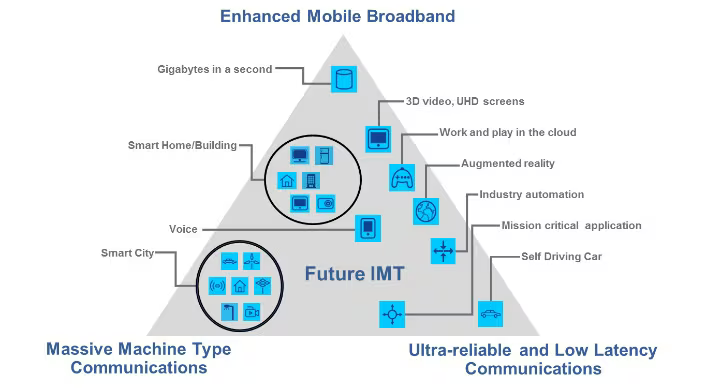
\includegraphics[width=\columnwidth]{itu-services.png}
    \caption{}
    \label{fig:service-types}
  \end{subfigure}
  \hfill
  \begin{subfigure}[b]{0.49\columnwidth}
    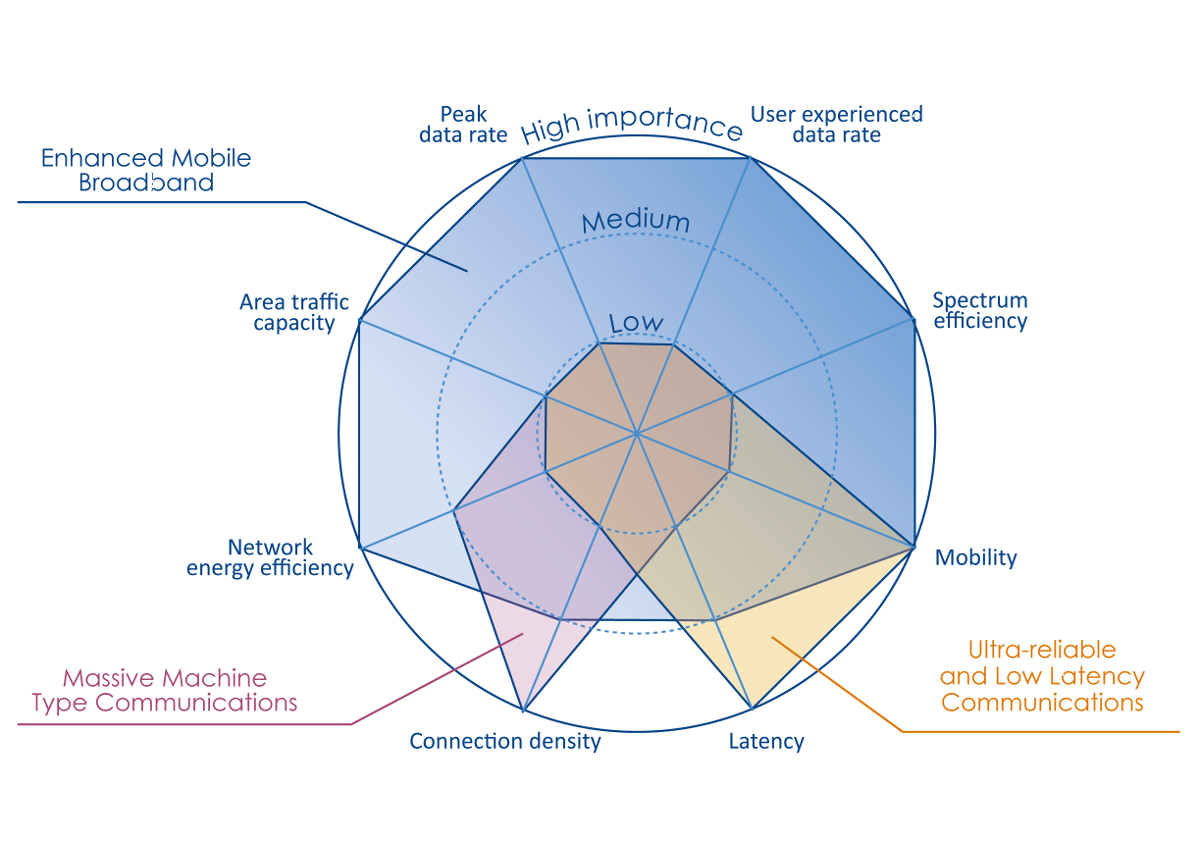
\includegraphics[width=\columnwidth]{spider-chart.png}
    \caption{}
    \label{fig:spider-chart}
  \end{subfigure}
  % \begin{subfigure}[b]{0.49\columnwidth}
  %   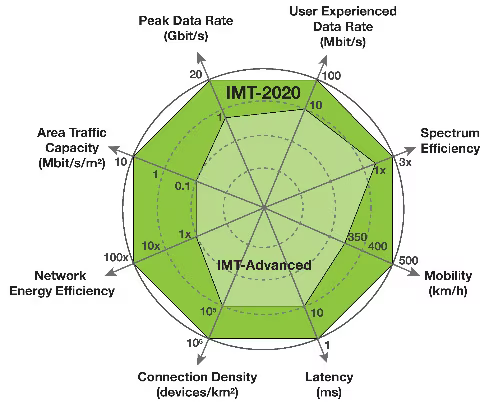
\includegraphics[width=\columnwidth]{itu-sevices-requirements.png}
  %   \caption{}
  %   \label{fig:service-requirements}
  % \end{subfigure}
  \caption{Different service types introduced for 5G: (a) examples of applications and (b) difference between requirements of eMBB, URLLC, and mMTC \cite{itu15m2083}.} %, and (c) comparison of 5G (IMT-2020) with 4G (IMT-Advanced) requirements
  \label{fig:plots}
\end{figure}

NS is the technology that utilizes softwarization and virtualization techniques across the MNO network in order to build logical networks tailored for each of the aforementioned service/slice types (see Fig. \ref{fig:slicing-overview}). The figure illustrates the virtualization of a physical network, enabling different types of slices to be supported by various virtualized elements such as virtual machines, containers, base stations, and routers, according to their specific requirements. For example, to support lower latency in the URLLC slice, the virtualized elements are pushed closer to the user in order to decrease propagation latency.

\begin{figure}
    \centering
    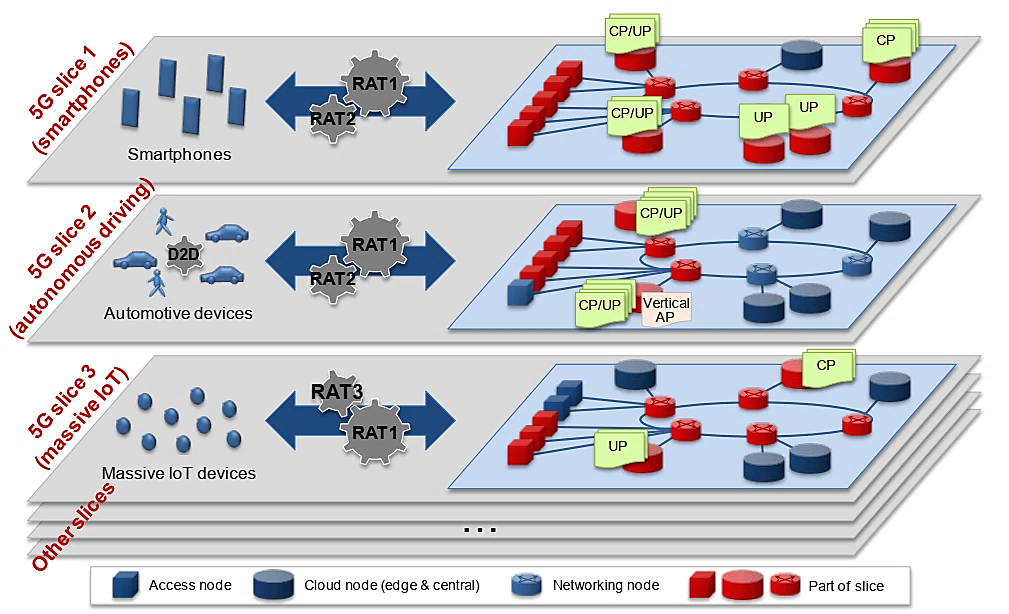
\includegraphics[width=0.7\columnwidth]{slicing-overview.png}
    \caption{Visual representation of the logical networks for different service/slice types in NS-enabled networks \cite{ngmn15wp5g}. User Plane (UP) and Control Plane (CP) network functions can be closer to the user to address certain requirements.}
    \label{fig:slicing-overview}
\end{figure}

This paper does not address the resource allocation process for NS. Instead, our focus is on forecasting the user's slice type by analyzing their characteristics. This can be done before the challenging and intricate process of resource allocation to support it. The source code of this paper is available in \href{https://github.com/sinaebrahimi/ml-7072cem}{Github}.

The next sections of this paper are organized as follows: The problem and dataset are introduced in Sec. \ref{dataset}. The various classification algorithms utilized in this paper are succinctly introduced in Sec. \ref{methods}. Sec. \ref{setup} and \ref{results} provide information about the experimental setup and the obtained results, respectively. Ultimately, the paper is concluded in Sec. \ref{conclusion}.

\section{Problem and Dataset} \label{dataset}%description (where you describe in detail the problem you want to solve and its significance)
The objective is to predict the slice type of the user (in the test set) based on the different characteristics outlined in the features. This can yield various advantages. For instance, this data can be utilized in the resource allocation mechanisms of 5G. By categorizing the user's slice type based on these characteristics, the algorithm will perform slice-aware resource allocation in the Radio Access Network (RAN) and/or Core Network (CN) for each user according to their slice type. Put simply, this exemplar algorithm depends on the slice type to determine the allocation of resources to the user.

This paper specifically examines the initial phase of the algorithm mentioned earlier. During this phase, we anticipate the users' slice type based on their characteristics, prior to the user initiating any signaling requests to the network controller to indicate their slice type. This information may be inaccessible for several reasons, such as the absence of slicing support in the User Equipment (UE). Another situation in which we could employ this categorization is to decrease the number of signaling messages exchanged between the user and the network, thereby minimizing user latency.

The dataset is acquired from the file \texttt{\footnotesize train\_dataset.csv} in the Kaggle repository titled \textit{'Network Slicing in 5G'} \cite{kaggle23kumar}. This dataset has 31,583 samples and 17 features in total with no missing values. Each sample is the characteristics and requirements of one specific end-user that has used 4G (LTE) or 5G service. The target variable is \texttt{\footnotesize Slice Type}, which classifies the selected slice type for the user within the network (See Table \ref{tab:slice-type}).

\begin{table}
    \centering
    \scriptsize
    \caption{Target variable ("Slice Type") and its meaning in communication services \cite{itu15m2083,kaggle23kumar}.}
    \begin{tabular}{l|l|l}
         Index in dataset& Service/slice type& Example use-case\\
         \hline
         1 & eMBB & AR/VR/Gaming services\\
         2 & URLLC & Remote surgery\\
         3 & mMTC & Smart metering (IoT)\\
    \end{tabular}
    \label{tab:slice-type}
    \vspace{-5mm}
\end{table}

The split of the train and test data is 70\% to 30\%. Moreover, as we are dealing with a classification problem, we need to check if our classes (see Table \ref{tab:slice-type} are balanced or not. Fig. \ref{fig:class-imbalance} shows the ratio of each slice type in the train dataset. We will proceed with classifying this imbalanced data, as it does not pose any issues for the algorithms. Put simply, the difference between the three classes is not significant enough to result in errors during the classification process.

\subsection{Features}
Table \ref{tab:features} shows the dataset features. Moreover, Table \ref{tab:statistical-information} shows the statistical attributes of all features in the train dataset. 

\begin{table}
    \centering
    \scriptsize
    \caption{Dataset Features}
    \begin{tabular}{p{0.15cm}|p{1.7cm}|p{1.25cm}|p{0.7cm}|p{4.1cm}}
        No. & Column name  & Data Type & Range & Description \\
        \hline
        1 & LTE/5g Category & Integer & 1-22 & No description in Dataset\\
        2 & Time & Integer & 0-23 & No description in Dataset\\
        3 & Packet Loss Rate & Float & 1e-6 to 1e-2 & Number of packets not received divided by the total number of packets sent \\
        4 & Packet delay & Integer & 10-300 & The time for a packet to be received (in ms) \\
        5 & IoT & Binary (Int.) & 0 \& 1 & No description in Dataset\\
        6 & LTE/5G & Binary (Int.) & 0 \& 1 & No description in Dataset\\
        7 & GBR & Binary (Int.) & 0 \& 1 & Guaranteed Bit Rate\\
        8 & Non-GBR & Binary (Int.) & 0 \& 1 & Non-Guaranteed Bit Rate\\
        9 & AR/VR/Gaming & Binary (Int.) & 0 \& 1 & No description in Dataset\\
        10 & Healthcare & Binary (Int.) & 0 \& 1 & Usage in Healthcare\\
        11 & Industry 4.0 & Binary (Int.) & 0 \& 1 & Usage in Digital Enterprises\\
        12 & IoT Devices & Binary (Int.) & 0 \& 1 & Usage of IoT devices\\
        13 & Public Safety & Binary (Int.) & 0 \& 1 & Usage for public welfare and safety purposes\\
        14 & Smart City \& Home & Binary (Int.) & 0 \& 1 & usage in daily household chores\\
        15 & Smart Transportation & Binary (Int.) & 0 \& 1 & usage in public transportation\\
        16 & Smartphone & Binary (Int.) & 0 \& 1 & whether used for smartphone cellular data\\
        \hline
        17 & Slice Type & Integer & 1-3 & 1: eMBB, 2: URLLC, 3: mMTC\\
    \end{tabular}
    \label{tab:features}
    \vspace{-5mm}
\end{table}


\setlength{\tabcolsep}{2pt}
\begin{table*}[htbp]
\centering
\scriptsize
\caption{Statistical information about the train dataset features.}
\label{tab:statistical-information}
\resizebox{\textwidth}{!}{
\begin{tabular}{lcccccccccccccccccc}
\toprule
\textbf{Meausre} & \textbf{\begin{tabular}[c]{@{}l@{}}LTE/5g\\ Category\end{tabular}} & \textbf{Time} & \textbf{\begin{tabular}[c]{@{}l@{}}Packet\\ Loss Rate\end{tabular}} & \textbf{Packet delay} & \textbf{IoT} & \textbf{LTE/5G} & \textbf{GBR} & \textbf{Non-GBR} & \textbf{\begin{tabular}[c]{@{}l@{}}AR/VR/\\ Gaming\end{tabular}} & \textbf{Healthcare} & \textbf{Industry 4.0} & \textbf{IoT Devices} & \textbf{Public Safety} & \textbf{\begin{tabular}[c]{@{}l@{}}Smart City\\ \& Home\end{tabular}} & \textbf{\begin{tabular}[c]{@{}l@{}}Smart\\ Transportation\end{tabular}} & \textbf{Smartphone} & \textbf{Slice Type} \\
\midrule
\textbf{count} & 31583 & 31583 & 31583 & 31583 & 31583 & 31583 & 31583 & 31583 & 31583 & 31583 & 31583 & 31583 & 31583 & 31583 & 31583 & 31583 & 31583 \\
\textbf{mean} & 10.97 & 11.48 & 0.00308 & 114.13 & 0.47 & 0.53 & 0.44 & 0.56 & 0.11 & 0.06 & 0.12 & 0.06 & 0.06 & 0.12 & 0.06 & 0.43 & 1.70 \\
\textbf{std} & 6.05 & 6.92 & 0.00434 & 106.32 & 0.50 & 0.50 & 0.50 & 0.50 & 0.31 & 0.23 & 0.32 & 0.23 & 0.24 & 0.32 & 0.24 & 0.49 & 0.82 \\
\textbf{min} & 1.0 & 0.0 & 1e-06 & 10.0 & 0.0 & 0.0 & 0.0 & 0.0 & 0.0 & 0.0 & 0.0 & 0.0 & 0.0 & 0.0 & 0.0 & 0.0 & 1.0 \\
\textbf{25\%} & 6.0 & 6.0 & 1e-06 & 50.0 & 0.0 & 0.0 & 0.0 & 0.0 & 0.0 & 0.0 & 0.0 & 0.0 & 0.0 & 0.0 & 0.0 & 0.0 & 1.0 \\
\textbf{50\%} & 11.0 & 11.0 & 0.001 & 75.0 & 0.0 & 1.0 & 0.0 & 1.0 & 0.0 & 0.0 & 0.0 & 0.0 & 0.0 & 0.0 & 0.0 & 0.0 & 1.0 \\
\textbf{75\%} & 16.0 & 17.0 & 0.01 & 150.0 & 1.0 & 1.0 & 1.0 & 1.0 & 0.0 & 0.0 & 0.0 & 0.0 & 0.0 & 0.0 & 0.0 & 1.0 & 2.0 \\
\textbf{max} & 22.0 & 23.0 & 0.01 & 300.0 & 1.0 & 1.0 & 1.0 & 1.0 & 1.0 & 1.0 & 1.0 & 1.0 & 1.0 & 1.0 & 1.0 & 1.0 & 3.0 \\
\bottomrule
\end{tabular}
}
\vspace{-5mm}
\end{table*}

\subsection{Correlation Analysis}
In order to determine the correlation between different features, we can utilize a correlation matrix, as depicted in Figs. \ref{fig:eda-plot-slice-type} and \ref{fig:eda-plot-slice-type-only}. There is a strong correlation between \texttt{\footnotesize IoT} and \texttt{\footnotesize Slice Type}. Furthermore, the features \texttt{\footnotesize Smartphone} and \texttt{\footnotesize LTE/5G} exhibit a robust negative correlation with \texttt{\footnotesize Slice Type}. Hence, these three characteristics hold great significance in determining the \texttt{\footnotesize Slice Type}. The features \texttt{\footnotesize LTE/5g Category}, \texttt{\footnotesize Time}, \texttt{\footnotesize Packet Loss Rate}, and \texttt{\footnotesize IoT Devices} have a weak correlation (i.e., between -0.1 and 0.1) with \texttt{\footnotesize Slice Type}. 
%Therefore, we remove these features from both the train and test datasets to reduce dimensionality.

\begin{figure}[!t]
    \centering
    \begin{subfigure}[b]{0.425\columnwidth}
        \centering
        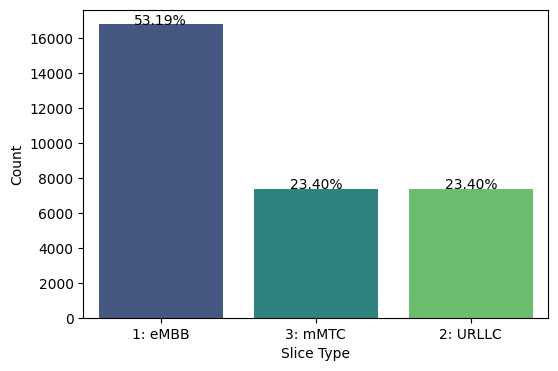
\includegraphics[width=\columnwidth]{class-imbalance.png}
        \caption{Class imbalance: ratio of each slice type in the train dataset.}
        \label{fig:class-imbalance}
    \end{subfigure}
    \hfill
    \begin{subfigure}[b]{0.562\columnwidth}
        \centering
        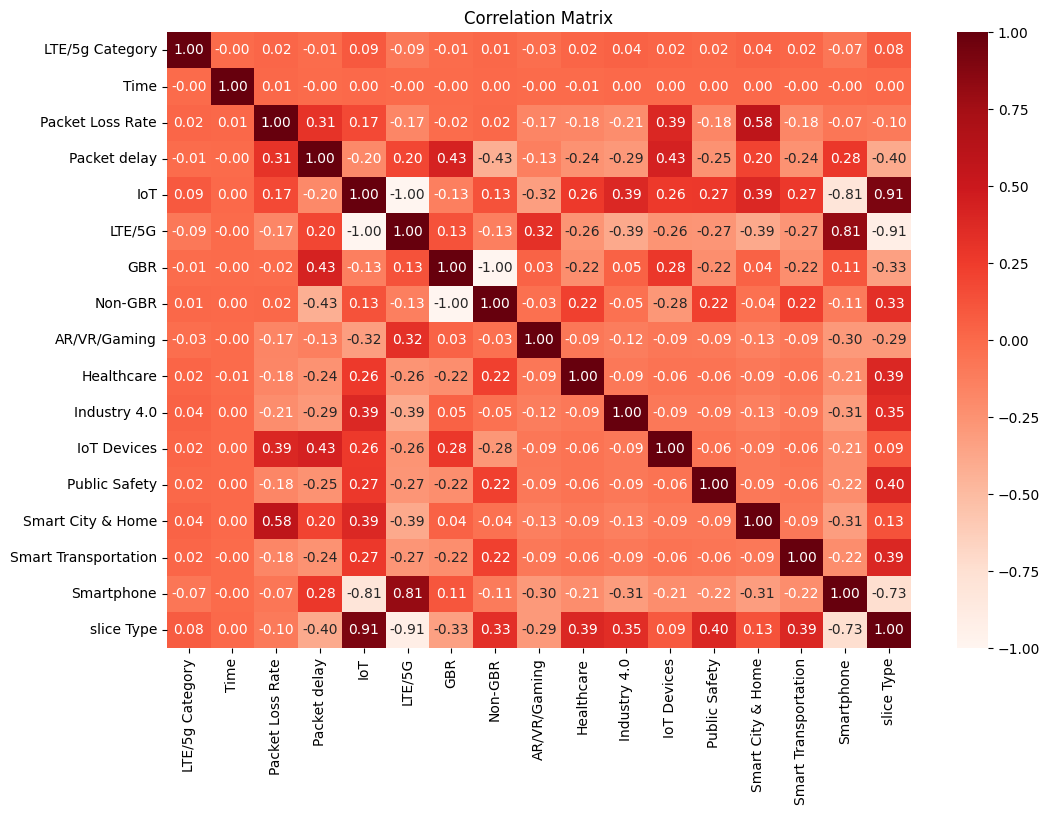
\includegraphics[width=\columnwidth]{eda-plot-slice-type-red.png}
        \caption{Correlation matrix for the train dataset.}
        \label{fig:eda-plot-slice-type}
    \end{subfigure}

    \begin{subfigure}[b]{0.9\columnwidth}
        \centering
        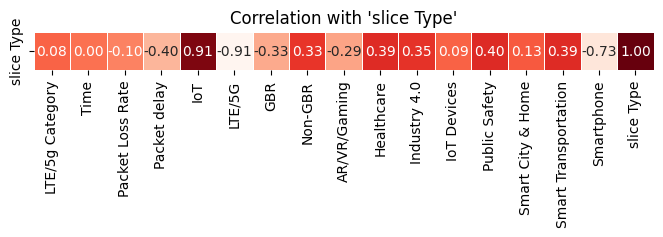
\includegraphics[width=\columnwidth]{eda-plot-slice-type-only-red.png}
        \caption{Correlation matrix only for the target variable (\texttt{\footnotesize Slice Type}).}
        \label{fig:eda-plot-slice-type-only}
    \end{subfigure}
    \caption{Class imbalance and correlation matrices.}
    \label{fig:correlation_class_imbalance}
\end{figure}

% \begin{figure}
%     \centering
%     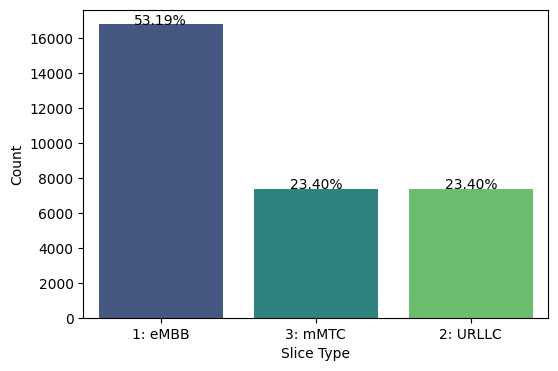
\includegraphics[width=0.5\columnwidth]{class-imbalance.png}
%     \caption{Class imbalance: ratio of each slice type in the train dataset.}
%     \label{fig:class-imbalance}
%     \vspace{-6mm}
% \end{figure}
% \begin{figure}
%     \centering
%     \begin{subfigure}[b]{\columnwidth}
%         \centering
%         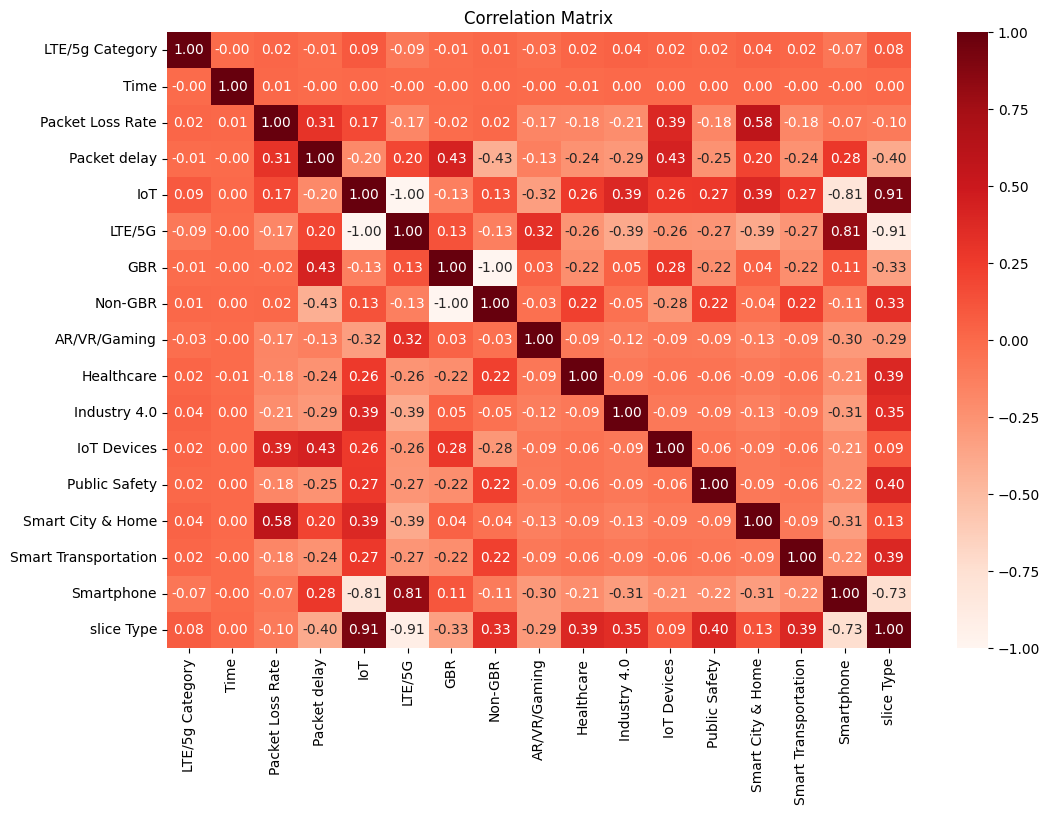
\includegraphics[width=0.7\columnwidth]{eda-plot-slice-type-red.png}
%         \caption{Correlation matrix for the train dataset.}
%         \label{fig:eda-plot-slice-type}
%     \end{subfigure}
%     \\
%     \begin{subfigure}[b]{\columnwidth}
%         \centering
%         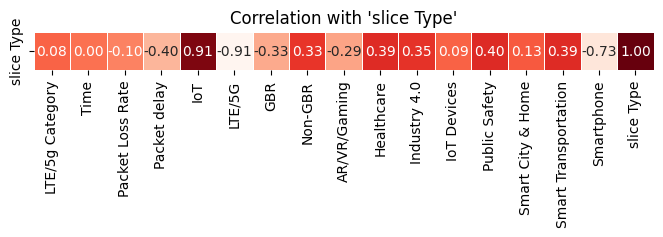
\includegraphics[width=0.6\columnwidth]{eda-plot-slice-type-only-red.png}
%         \caption{Correlation matrix only for the target variable (slice type).}
%         \label{fig:eda-plot-slice-type-only}
%     \end{subfigure}
%     \caption{Correlation matrices.}
% \end{figure}

% \begin{figure}
%     \centering
%     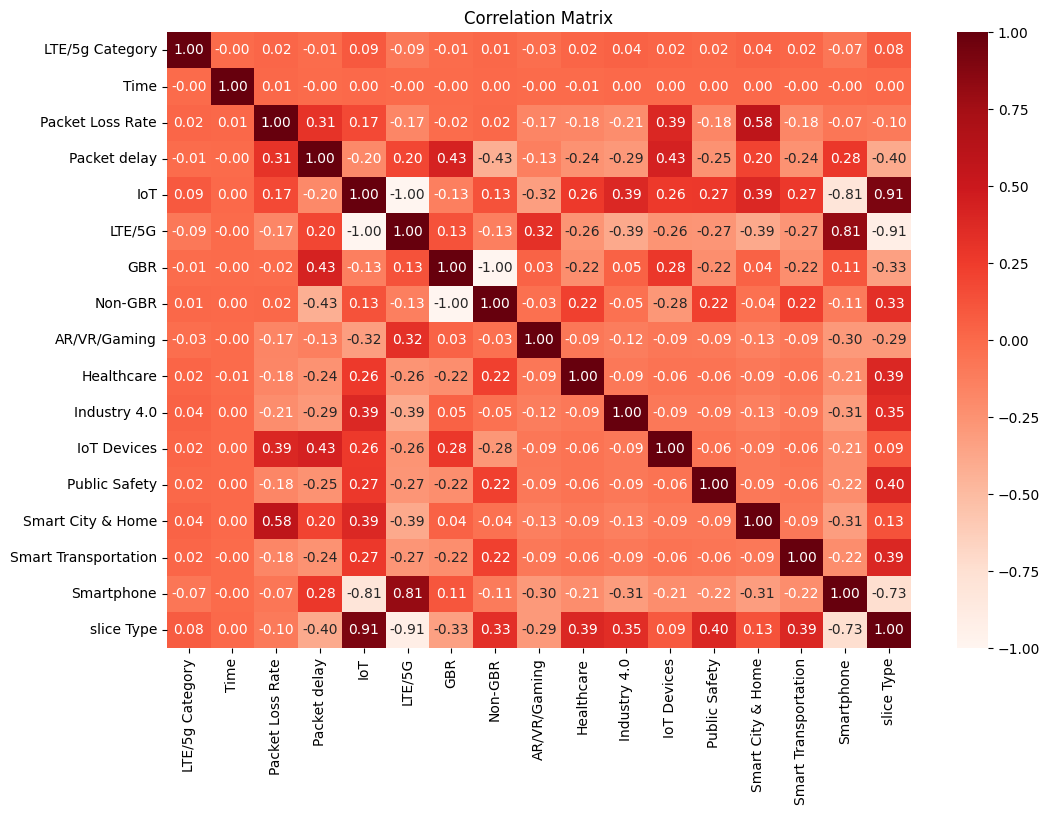
\includegraphics[width=\columnwidth]{eda-plot-slice-type-red.png}
%     \caption{Correlation matrix for the train dataset (slice type is dropped).}
%     \label{fig:eda-plot-slice-type}
% \end{figure}

% \begin{figure}
%     \centering
%     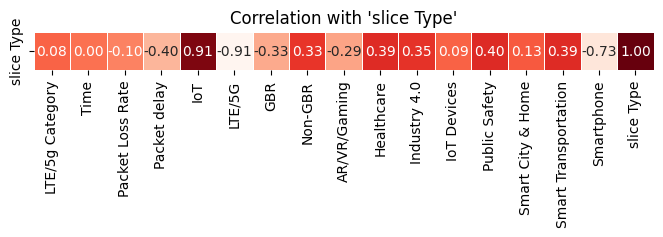
\includegraphics[width=\columnwidth]{eda-plot-slice-type-only-red.png}
%     \caption{Correlation matrix only for the target variable (slice type)).}
%     \label{fig:eda-plot-slice-type-only}
% \end{figure}

\subsection{Feature Selection}
According to the 3GPP TS 22.261 standard \cite{3gpp23ts22261}, during the registration period, each UE only transmits specific information to the CN. This information includes the \texttt{\footnotesize LTE/5g Category}, \texttt{\footnotesize Time}, \texttt{\footnotesize Packet Loss Rate}, \texttt{\footnotesize Packet Delay}, and \texttt{\footnotesize Healthcare}. This dataset contains an additional 11 features in addition to the \texttt{\footnotesize Slice Type} feature. However, in practical situations where we need to assign resources to the user according to their slice type, we lack access to the remaining 11 features during the UE registration period. Hence, it is imperative to forecast the type of slice by utilizing the aforementioned 5 features and subsequently execute our resource allocation algorithm. Since we have a limited number of features (only 5), there is no necessity to apply dimensionality reduction techniques like Principal Component Analysis (PCA) to the data.

%Packet loss rate should be transformed to integer values. For example, 0.001, i.e., 1e-3, should be transformed to 3 and 1e-6 should be converted to 6. Therefore, the higher this value is, the tighter and harder to achieve this requirement is.
\subsection{Ethics}
The dataset under examination is devoid of personal data and has been anonymized, thus eliminating the risk of personal data leakage through its analysis. The data is sourced from various entries in tables within Mobile MNO's CN databases. Standardization protocols ensure that the primary keys within these tables are anonymized. Identification of users based on these keys necessitates additional access to other CN functions, which is not granted to third parties. Furthermore, these primary keys are absent from the dataset’s features and have been duly sanitized.

\section{Methods} \label{methods}%where you shortly describe the machine learning methods and/or other methods employed to solve the problem
For this problem, we can use multi-class classification algorithms from the supervised learning schemes as we have 3 discrete target variables (see Fig. \ref{fig:class-imbalance}). Different classification algorithms are introduced in this section.

\subsection{Decision Tree (DT)}
The DT algorithm is a non-parametric supervised learning method that is commonly employed for both classification and regression tasks. The model's interpretability and capacity to handle both categorical and numerical data make it well-suited for predicting the \texttt{\footnotesize Slice Type} in our dataset. The hyperparameter \texttt{\footnotesize max\_depth} governs the upper limit on the depth of the tree, thereby influencing the complexity of the model. A higher value for the \texttt{\footnotesize max\_depth} parameter allows for more information to be captured, but there is a risk of overfitting the data. Conversely, a lower value for \texttt{\footnotesize max\_depth} may result in the data being underfit. 

Fig. \ref{fig:dt} displays the various scores and execution times of the DT algorithm for different values of the hyperparameter \texttt{\footnotesize max\_depth}, ranging from 1 to 9. The analysis indicates that the ideal value for \texttt{\footnotesize max\_depth} is 4. Higher \texttt{\footnotesize max\_depth} will result in overfitting and also higher execution time. Therefore, we will use this algorithm with \texttt{\footnotesize max\_depth=4} in the next sections.

\begin{figure}
    \centering
    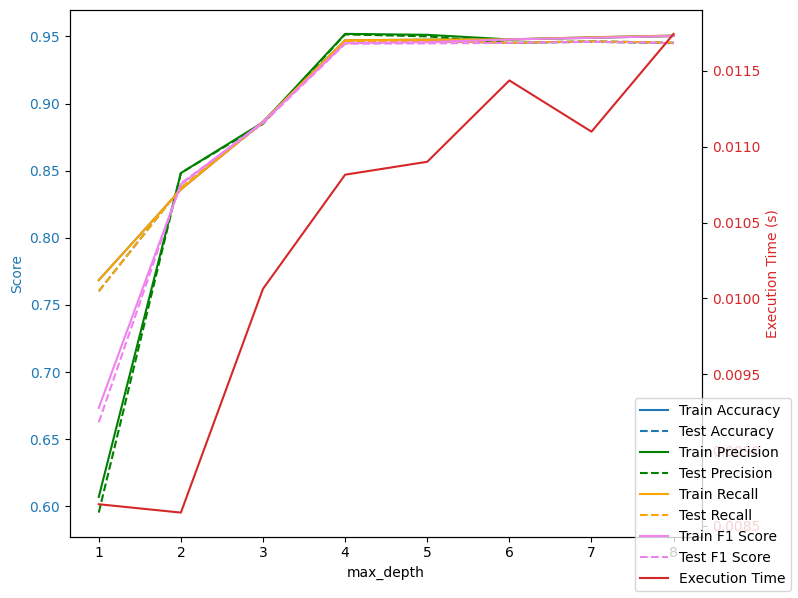
\includegraphics[width=0.55\columnwidth]{dt_max_depth.png}
    \caption{Evaluating accuracy, precision, recall, F1 score, and execution time for different \texttt{\footnotesize max\_depth} values in DT.}
    \label{fig:dt}
\end{figure}

\subsection{Random Forest (RF)}
The RF algorithm is a technique used in ensemble learning for both classification and regression tasks. It operates by creating numerous DTs during the training process and determining the class that appears most frequently (for classification, which is our case). RFs mitigate the tendency of DTs to overfit their training set. They effectively decrease the variability of the DT estimator by averaging multiple DTs, each grown to its maximum depth on bootstrap samples of the training data. The introduction of randomness during the tree construction process leads to the trees becoming less correlated with each other, which ultimately improves their predictive performance. The hyperparameter \texttt{\footnotesize n\_estimators} determines the quantity of trees present in the forest. In general, a greater quantity of trees enhances performance and improves the stability of predictions, although it does result in slower computation.

In our case, after examining Fig. \ref{fig:rf}, we have selected the value of 15 for \texttt{\footnotesize n\_estimators}. This value represents an optimal balance between computational efficiency and model performance, yielding a robust and precise model for predicting the \texttt{\footnotesize Slice Type} in our dataset.

\begin{figure}[!t]
    \centering
    \begin{subfigure}[b]{0.49\columnwidth}
        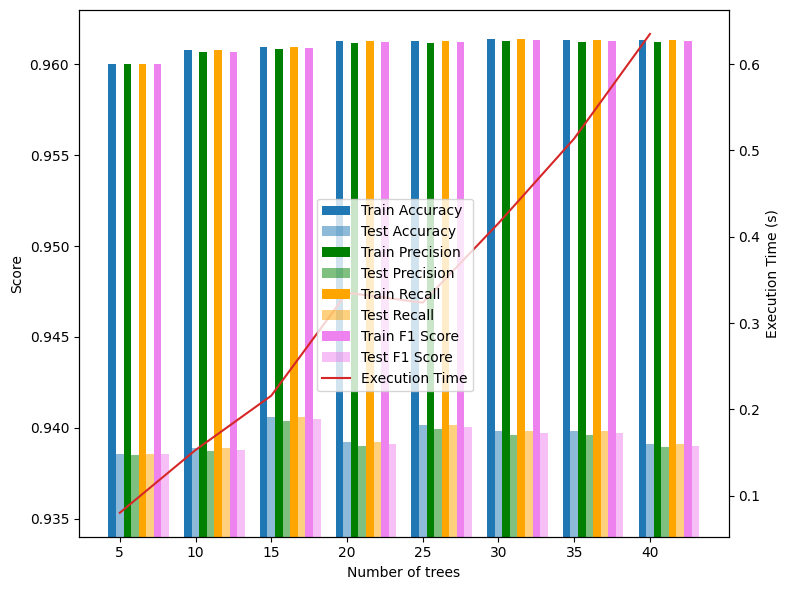
\includegraphics[width=\textwidth]{rf_n_estimators.png}
        \caption{RF}\label{fig:rf}
    \end{subfigure}
    \hfill
    \begin{subfigure}[b]{0.49\columnwidth}
        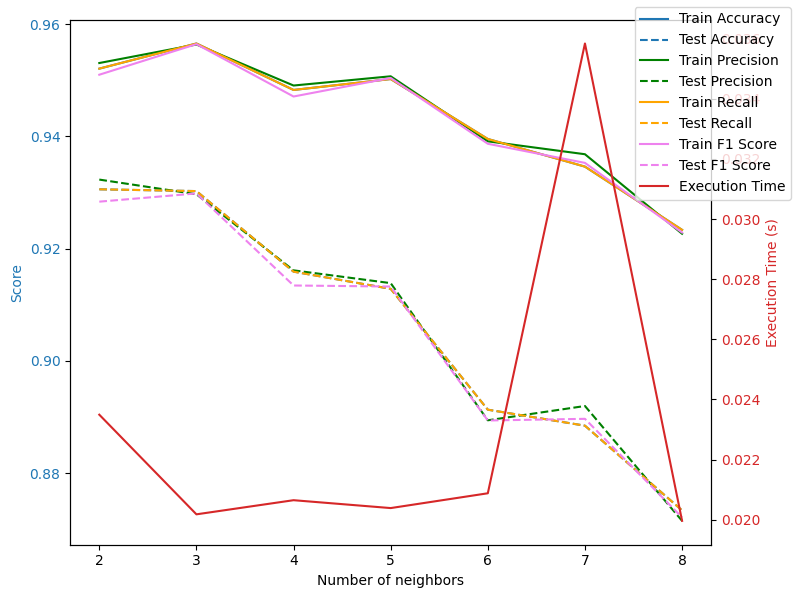
\includegraphics[width=\textwidth]{knn_n_neighbors.png}
        \caption{KNN}\label{fig:knn}
    \end{subfigure}
    \vspace{-3mm}
    
    \begin{subfigure}[b]{0.49\columnwidth}
        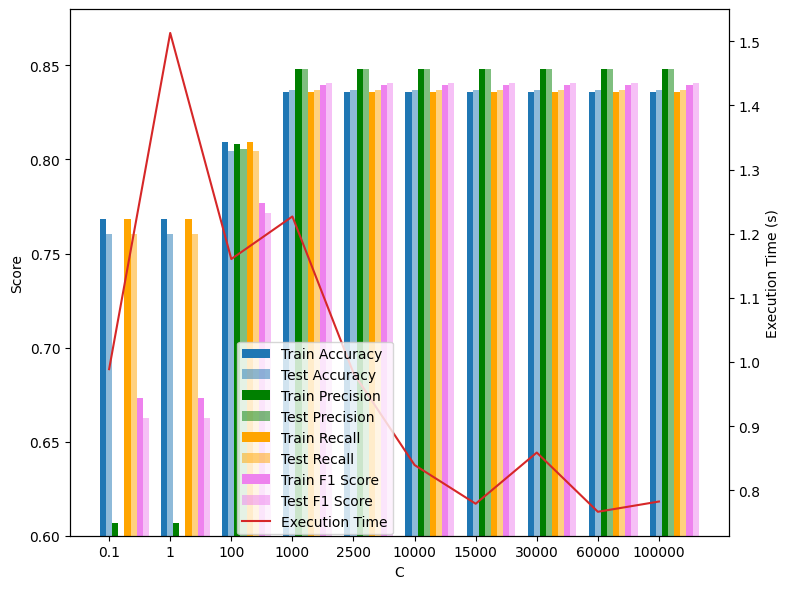
\includegraphics[width=\textwidth]{lr_c.png}
        \caption{LR}\label{fig:lr}
    \end{subfigure}
    \hfill
    \begin{subfigure}[b]{0.49\columnwidth}
        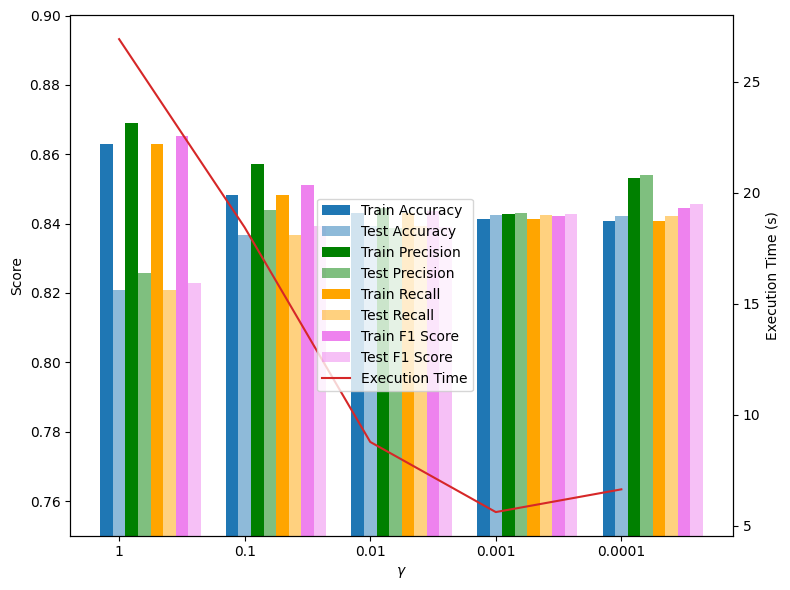
\includegraphics[width=\textwidth]{svm_gamma.png}
        \caption{SVM}\label{fig:svm}
    \end{subfigure}
    \caption{Evaluating accuracy, precision, recall, F1 score, and execution time for various (a) \texttt{\footnotesize n\_estimators} values in RF, (b) \texttt{\footnotesize n\_neighbors} values in KNN, (c) \texttt{\footnotesize C} values in LR, and (d) \texttt{\footnotesize gamma} values in SVM.}
    \label{fig:rf_knn_lr_svm_hyperparameters}
    \vspace{-5mm}
\end{figure}

\subsection{K-Nearest Neighbors (KNN)}
The KNN algorithm is a form of instance-based learning technique employed for both classification and regression problems. It functions by storing all existing cases and classifying new instances using a similarity measure (e.g., Manhattan distance). KNN possesses the benefit of being straightforward, comprehensible, and having a broad range of applications. It is applicable to multi-class problems and is resistant to noisy training data. Nevertheless, it can be resource-intensive and necessitate the normalization of the input features. The hyperparameter \texttt{\footnotesize n\_neighbors} determines the number of neighboring data points to take into account during the prediction process. A lower value of \texttt{\footnotesize n\_neighbors} increases the susceptibility of predictions to noise, whereas a higher value of \texttt{\footnotesize n\_neighbors} enhances the stability of predictions by reducing the impact of noise but may result in decreased accuracy.

After analyzing Fig. \ref{fig:knn}, we have selected the value of \texttt{\footnotesize n\_neighbors} to be 3 in our case. This value achieves a favorable equilibrium between accurately representing the subtleties in the data and preventing overfitting caused by noise or outliers. Therefore, it provides a strong and precise model for forecasting the \texttt{\footnotesize Slice Type} in our dataset.

\subsection{Logistic Regression (LR)}
LR is a binary classification model that can be adapted to handle multi-class problems via the one-vs-rest (OvR) strategy. In OvR, a distinct model is trained for each class, with the objective of distinguishing that class from all other classes. This transforms the problem into a binary classification task. In order to address our three-class problem, we proceed by training three separate models, each one specifically designed to classify one slice type against the remaining classes. The parameter \texttt{\footnotesize C} in LR determines the strength of regularization and should be a positive floating-point number. Lower values indicate more pronounced regularization. Regularization involves imposing a penalty on the amplification of parameter values to mitigate overfitting. When training a model, such as LR, on a dataset, there is a possibility that the model may exhibit overfitting to the training data. Regularization mitigates overfitting by penalizing excessively intricate models in a manner that aligns with natural tendencies.

After analyzing Fig. \ref{fig:lr}, we have determined that the value of \texttt{\footnotesize C} is 15000 in our situation. This value represents an optimal balance between the problem of underfitting and the problem of overfitting. By selecting the value of \texttt{\footnotesize C} in this manner, our model possesses sufficient adaptability to accurately capture the data while avoiding excessive adaptation to the noise present in the data. Therefore, it provides a strong and precise model for predicting the \texttt{\footnotesize Slice Type} in our dataset.

\subsection{Support Vector Machine (SVM)} % Not enough space... also, its scores were around 82% (much lower than others)
SVM is a robust ML model used for both classification and regression. It operates by identifying the hyperplane that best divides the classes in the feature space. For a multi-class classification problem with three classes, SVM can be expanded using techniques such as One-vs-Rest (OvR) or One-vs-One (OvO). In our problem, we utilize the OvR approach, the default method in scikit-learn \cite{scikit-learn}, as it demonstrates a slight advantage over the OvO method. The \texttt{\footnotesize gamma} parameter in SVM determines the extent to which a single training example affects the model, with low values indicating a wider influence and high values indicating a narrower influence. Put simply, it is a parameter for non-linear hyperplanes, and the higher the \texttt{\footnotesize gamma} value, the more it tries to exactly fit the training data set.
%For non-linearly separable data, SVM uses a technique called the kernel trick to project the data into a higher-dimensional space where it is linearly separable.

Upon analyzing our data and carefully weighing the trade-off between bias and variance, we have selected a value of 0.0001 for \texttt{\footnotesize gamma} in our SVM model (see Fig. \ref{fig:svm}. This value achieves a favorable equilibrium, enabling the model to precisely categorize the \texttt{\footnotesize Slice Type} in our dataset without succumbing to overfitting.

\section{Experimental Setup} \label{setup}%including data pre-processing, feature selection and extraction, classification/clustering parameters
The primary component of the project, which involves classification algorithms, utilizes the scikit-learn library \cite{scikit-learn}. This library offers the necessary functions for programming in the Python language. Google Colab is used to execute the codes. The next section compares the results of different algorithms briefly introduced in Sec. \ref{methods} in our prediction problem.

\section{Results} \label{results}
This section compares the five different multi-class classifiers introduced in Sec. \ref{methods}. The hyperparameters used for each of the algorithms are listed in Table \ref{tab:hyperparameters}. Besides these hyperparameters, other options and hyperparameters are the default ones in the scikit-learn library.


\begin{table}
    \caption{Modified hyperparameters in each algorithm.}
    \centering
    \begin{tabular}{l|l|l}
        Algorithm & Hyperparameter & Value\\
        \hline
        DT & \texttt{\small max\_depth} & 4\\
        RF & \texttt{\small n\_estimators} & 15\\
        KNN & \texttt{\small n\_neighbors} & 3\\
        LR & \texttt{\small C} & 15000\\
        SVM & \texttt{\small gamma} & 0.0001\\
    \end{tabular}
    \label{tab:hyperparameters}
    \vspace{-5mm}
\end{table}

\subsection{Classification Reports}
A classification report is a metric used to evaluate the performance of an ML model. This metric is employed to display the precision, recall, F1-score, and support for each class within your model. The following is an explanation of each term:
\begin{itemize}
    \item \textbf{Precision} is the proportion of accurately predicted positive observations out of all the predicted positives. The question it addresses is "\textit{What is the accuracy rate of positive identifications?}"
    \item \textbf{Recall} (sensitivity) refers to the proportion of accurately predicted positive observations out of all the actual positive observations. The question it addresses is "\textit{What is the accuracy rate of correctly identifying actual positives?}"
    \item \textbf{F1-Score} is a metric that calculates the weighted average of precision and recall. It endeavors to achieve a trade-off between precision and recall.
    \item \textbf{Support} refers to the count of the actual instances of the class within the given dataset. If there is an uneven distribution of support in the training data, it could mean that the classifier's reported scores are wrong and that you need to use stratified sampling or rebalancing techniques.
\end{itemize}

The classification report provides a thorough overview of the model's performance, with a detailed breakdown for each class. Table \ref{tab:classification_reports} displays the classification report for all the algorithms utilized. The output offers a comprehensive analysis of the performance of each classifier in terms of precision, recall, F1-score, and support. The report indicates that categorizing the third class (referred to as \texttt{\footnotesize Slice Type='mMTC'}) is relatively simple for all of the algorithms when utilizing the chosen five features. The DT, RF, and KNN algorithms exhibit superior performance compared to the LR and SVM methods, making them more suitable for our classification problem.

\begin{table}[h]
\vspace{-3mm}
\centering
\caption{Classification Reports for the five evaluated classifiers.}
\label{tab:classification_reports}
\begin{tabular}{|l|l|l|l|l|}
\hline
\multicolumn{5}{|c|}{\textbf{DT}} \\ \hline
& Precision & Recall & F1-Score & Support \\ \hline
1 & 0.91 & 1.00 & 0.95 & 5007 \\ \hline
2 & 1.00 & 0.78 & 0.87 & 2272 \\ \hline
3 & 1.00 & 1.00 & 1.00 & 2196 \\ \hline \hline
\multicolumn{5}{|c|}{\textbf{RF}} \\ \hline
& Precision & Recall & F1-Score & Support \\ \hline
1 & 0.94 & 0.95 & 0.94 & 5007 \\ \hline
2 & 0.88 & 0.87 & 0.88 & 2272 \\ \hline
3 & 1.00 & 1.00 & 1.00 & 2196 \\ \hline \hline
\multicolumn{5}{|c|}{\textbf{KNN}} \\ \hline
& Precision & Recall & F1-Score & Support \\ \hline
1 & 0.93 & 0.94 & 0.93 & 5007 \\ \hline
2 & 0.87 & 0.83 & 0.85 & 2272 \\ \hline
3 & 1.00 & 1.00 & 1.00 & 2196 \\ \hline \hline
\multicolumn{5}{|c|}{\textbf{LR}} \\ \hline
& Precision & Recall & F1-Score & Support \\ \hline
1 & 0.86 & 0.82 & 0.84 & 5007 \\ \hline
2 & 0.63 & 0.71 & 0.67 & 2272 \\ \hline
3 & 1.00 & 1.00 & 1.00 & 2196 \\ \hline \hline
\multicolumn{5}{|c|}{\textbf{SVM}} \\ \hline
& Precision & Recall & F1-Score & Support \\ \hline
1 & 0.89 & 0.80 & 0.84 & 5007 \\ \hline
2 & 0.64 & 0.77 & 0.70 & 2272 \\ \hline
3 & 1.00 & 1.00 & 1.00 & 2196 \\ \hline
\end{tabular}
\vspace{-5mm}
\end{table}

\subsection{Confusion Matrix}
A confusion matrix is a tabular representation commonly employed in ML to visually depict the effectiveness of a classification algorithm. The matrix is structured such that each row corresponds to the instances in a predicted class, and each column corresponds to the instances in an actual class. In a three-class problem, the $3\times3$ matrix displays accurate and inaccurate predictions for each class. Greater diagonal values indicate a higher number of accurate predictions. 

The confusion matrix for each of the assessed algorithms is illustrated in Figure \ref{fig:confusion_matrices}. The results indicate that the DT algorithm outperforms RF and KNN in classifying the first class, with only 506 incorrect classifications compared to 558 and 661, respectively. DT outperforms KNN and RF in the second class. All classifiers are equally capable of identifying the third class. Moreover, it is evident that the performance of the LR and SVM algorithms is noticeably lower than the other three classifiers.

\begin{figure}[!t]
    \centering
    \begin{subfigure}[b]{0.32\columnwidth}
        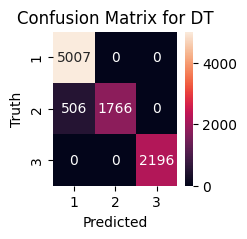
\includegraphics[width=\textwidth]{confusion_matrix_dt.png}
        \caption{DT}\label{fig:cm_dt}
    \end{subfigure}
    \hfill
    \begin{subfigure}[b]{0.32\columnwidth}
        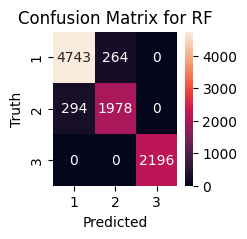
\includegraphics[width=\textwidth]{confusion_matrix_rf.png}
        \caption{RF}\label{fig:cm_rf}
    \end{subfigure}
    \hfill
    \begin{subfigure}[b]{0.32\columnwidth}
        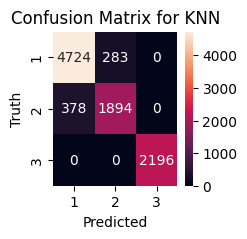
\includegraphics[width=\textwidth]{confusion_matrix_knn.png}
        \caption{KNN}\label{fig:cm_knn}
    \end{subfigure}
    \medskip
    
    \begin{subfigure}[b]{0.32\columnwidth}
        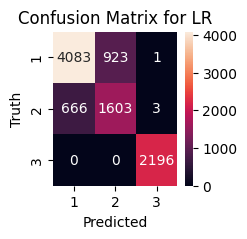
\includegraphics[width=\textwidth]{confusion_matrix_lr.png}
        \caption{LR}\label{fig:cm_lr}
    \end{subfigure}
    \hfill
    \begin{subfigure}[b]{0.32\columnwidth}
        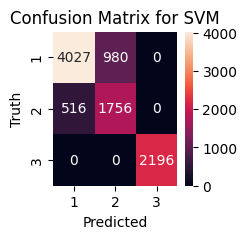
\includegraphics[width=\textwidth]{confusion_matrix_svm.png}
        \caption{SVM}\label{fig:cm_svm}
    \end{subfigure}
    \caption{Confusion matrices for the five classifiers.}
    \label{fig:confusion_matrices}
    \vspace{-5mm}
\end{figure}

\subsection{Evaluation of Different Scores}
This section compares different algorithms in terms of accuracy, average precision, average recall, average F1 score, and execution time.

Accuracy is a measure that quantifies the overall number of accurate predictions made by a model across all types of predictions. Accuracy is defined as the proportion of correctly predicted observations to the total number of observations. Fig. \ref{fig:accuracy} illustrates a comparison of the accuracy of the five classifiers. The DT model has an accuracy of 0.95, surpassing the RF and KNN models by 1\% and 2\%, respectively. SVM and LR exhibit lower levels of accuracy, with SVM achieving an accuracy of 0.84, a mere 1\% improvement over LR.

\begin{figure}
    \centering
    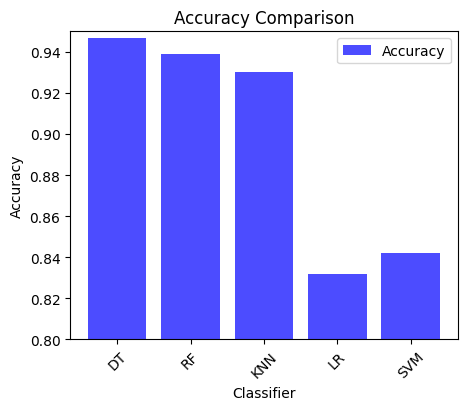
\includegraphics[width=0.6\columnwidth]{accuracy_comparison.png}
    \caption{Evaluating accuracy in different algorithms.}
    \label{fig:accuracy}
    \vspace{-6mm}
\end{figure}

For a classification problem with three classes, we can assess the effectiveness of our models by calculating the mean precision, recall, and F1-score. These metrics are computed for each individual class, and subsequently, a weighted average is computed to address the issue of class imbalance.

The precision metric can be calculated as an average in a multi-class classification problem. The precision of each class is calculated and then weighted by the number of true instances for each class to obtain the weighted average precision. Fig. \ref{fig:precision} shows the average precision in our models. The DT algorithm outperforms the RF and KNN algorithms by a margin of 1\% and 2\%, respectively.

\begin{figure}[h]
\centering
\subfloat[]{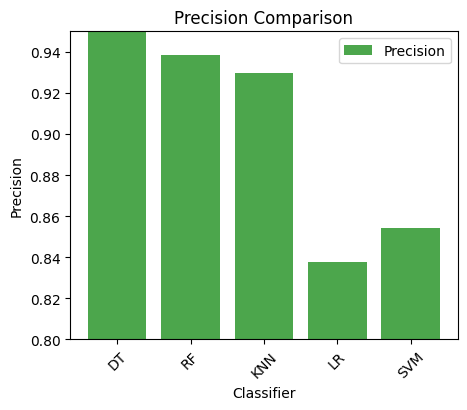
\includegraphics[width=0.22\textwidth]{precision_comparison.png}\label{fig:precision}}
\hfill
\subfloat[]{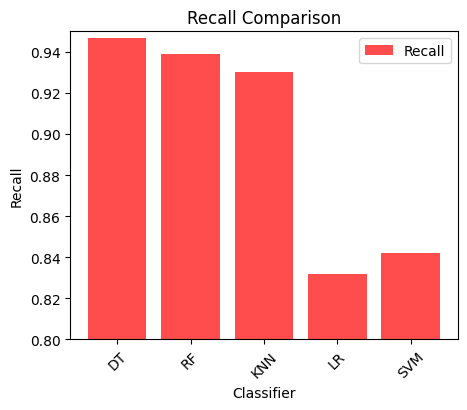
\includegraphics[width=0.22\textwidth]{recall_comparison.png}\label{fig:recall}}
\\
\subfloat[]{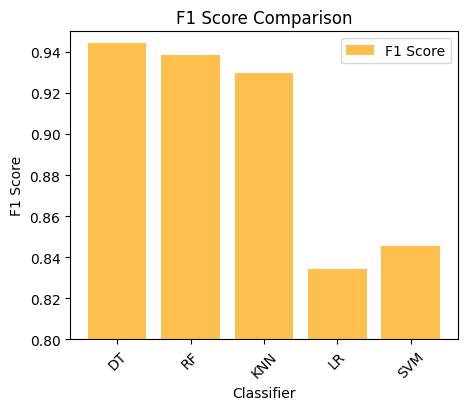
\includegraphics[width=0.22\textwidth]{f1_score_comparison.png}\label{fig:f1_score}}
\hfill
\subfloat[]{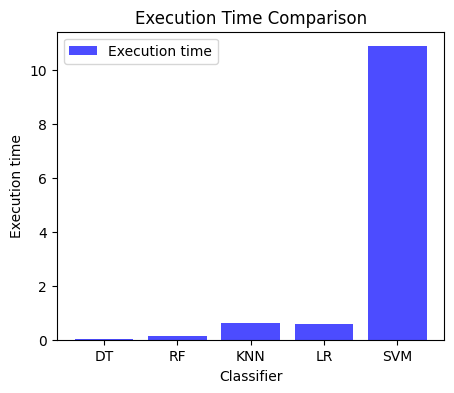
\includegraphics[width=0.22\textwidth]{execution_time_comparison.png}\label{fig:execution_time}}
\caption{Evaluation of the average (a) precision, (b) recall, (c) F1 score, and (d) execution time among the five classifiers.}
\label{fig:metrics}
    \vspace{-4mm}
\end{figure}

Similarly, the process of averaging can also be applied to recall. The metric represents the calculated average of the recall value for each individual class, taking into account their respective weights. Fig. \ref{fig:recall} depicts a comparison of the average recall for the five classifiers. The DT has a recall rate of 95\%, which is superior to the recall rates of RF, KNN, LR, and SVM by 1\%, 2\%, 11\%, and 9\%, respectively.

The F1 score can be computed using the same method of averaging. It generates a unified score that considers both precision and recall, resulting in a single numerical value. Fig. \ref{fig:f1_score} displays the average F1 score of our models. DT has a marginal advantage of less than 1\% compared to RF and less than 2\% compared to KNN. The SVM achieves an F1 score of 85\%, which is 9\% lower than the DT. However, the SVM achieves a mere 2\% improvement compared to the LR.

The execution time of the classifiers is another crucial metric that is used to determine the optimal balance between various algorithms. The execution time of each algorithm is measured by considering both the fitting and predicting processes. Fig. \ref{fig:execution_time} shows the duration of each algorithm's execution. The data indicates that the SVM algorithm is significantly more computationally intensive compared to other algorithms, taking 10.88 seconds to complete. This is approximately 777 times slower than the DT classifier, which is the most efficient algorithm with an execution time of only 14 ms. The RF algorithm, which has a runtime of 139 ms, is the second most efficient algorithm. However, it is still ten times slower than the DT algorithm, which is the simplest algorithm but also the most effective one for this particular problem. LR has a completion time of 567 milliseconds, whereas KNN takes approximately 633 milliseconds to finish. To summarize, the DT algorithm outperforms other algorithms in terms of execution time in this classification problem.

In conclusion, we can rank the algorithms in the following order: 1) DT, 2) RF, 3) KNN, 4) LR, and 5) SVM. DT has a slight advantage compared to RF and KNN in terms of accuracy as well as the average precision, recall, and F1 score. However, because of its simplicity, it is over 10 times faster than both of these classifiers, and therefore, it is chosen as the optimal algorithm for this classification problem.

\section{Discussion and Conclusions} \label{conclusion}
Accurately determining the appropriate slice type for the end-user is a crucial issue in wireless networks, as it directly impacts resource allocation. Accurately predicting outcomes leads to improved service quality for the end-user. This paper examines a dataset containing 16 characteristics and identifies 5 features that were chosen because of limitations in standardization. The data is divided into a 70\% training set and a 30\% testing set. Various classifiers, including DT, RF, KNN, LR, and SVM, can be employed for this discrete 3-class prediction problem. We optimized a hyperparameter for each classifier, choosing it based on a balance between various scores and execution times. Next, the algorithms are evaluated by using the scikit-learn library in Python. The findings indicate that the basic DT, with a depth of 4, surpasses other algorithms in terms of accuracy, achieving a rate of 95\%. It attains an accuracy, precision, recall, and F1 score that are approximately 1\% and 2\% higher than RF and KNN. However, it surpasses them in terms of execution time by being more than 10 times faster. Advanced techniques like SVM and LR not only exhibit slow execution times but also demonstrate inferior performance for this particular problem. 

A potential future endeavor involves developing a resource allocation mechanism for the 5G wireless network that utilizes reinforcement learning. This mechanism would allocate different resources, such as computation and bandwidth, to end-users based on the predicted slice type. Our low-complexity DT-based prediction method has the potential to be used for resource allocation in different slice types, as the quantity and type of resources can vary.

\bibliographystyle{ieeetr} 
\bibliography{main}{}

\appendix
The source code is available in a public \href{https://github.com/sinaebrahimi/ml-7072cem}{Github repository}. One should first navigate to the folder \texttt{\footnotesize Classifying Network Slices Based on User Requirements}. The dataset used is \texttt{\footnotesize train\_dataset.csv}. Preprocessing and analysis of the data are done in \texttt{\footnotesize preprocessing\_and\_analysis.ipynb}, and assessments of different algorithms are conducted in \texttt{\footnotesize prediction-final.ipynb}.
\end{document}
